\documentclass{beamer}
\mode<presentation>
{ \usetheme{boxes} }

\usepackage{times}
\usepackage{graphicx}
\usepackage[backend=bibtex]{biblatex}
\usepackage{verbatim}
% \addbibresourse{an_introduction_to_dogen.bib}

\title{Using Watertight Polygon Meshes for Neuronal Morphology Representation}

\subtitle{(or A Quixotic Quest for a Science Question)}
\author{
  \texorpdfstring
      {\href{mailto:marco.craveiro@gmail.com}{Marco Craveiro}}
      {Marco Craveiro}
}
\date{\today}

\AtBeginSection[]
{
  \begin{frame}<beamer>
    \frametitle{Outline}
    \tableofcontents[currentsection]
  \end{frame}
}

\bibliography{watertight}

\begin{document}

\begin{frame}
\titlepage
\end{frame}

\begin{frame}
\frametitle{Outline}
\begin{itemize}
\item SWC format
\pause
\item Polygon meshes
\pause
\item Processing Pipeline (code structure)
\pause
\item Problems and Solutions
\pause

\item Questions / Discussion
\end{itemize}
\end{frame}

\begin{frame}[fragile]
\frametitle{SWC}

\begin{itemize}

\item \emph{De facto} standard for storing morphology data.
\pause
\item The data is stored as a tree.
\pause
\item The internal format is a set of frusta (truncated cones),
  connected together in a parent and child relationship.
\pause
\item Powerful: morphometric work can be carried out from this simple
  tree representation, as per the functions provided by TREES and
  TREES2. Also useful for electrophysiology models, etc.
\pause
\end{itemize}

\begin{verbatim}
# id,type,x,y,z,r,pid
1 1 305.7912 312.7696 31.92 8.059 -1
2 2 307.4752 319.1016 31.9197 0.1144 1
3 2 307.7989 320.1896 31.8424 0.1731 2
5 2 309.0413 322.0349 31.7724 0.2652 4
...
\end{verbatim}
\end{frame}

\begin{frame}
\frametitle{SWC: Motivation for replacing}

SWC is a good format which has withstood the test of time, but has
some important shortcomings.
\pause

\begin{itemize}
\item Microscopy has improved dramatically but the resolution SWC
  provides is frusta: all of the high-resolution detail is lost in the
  final representation.
\pause
\item Loss of detail is applicable to both soma and the dendrites: the
  soma is represented as a sphere or a similar solid; the dendrites
  may miss dendritic spines altogether or have very inaccurate
  representations.
\pause
\item SWC was designed in the nineties, where computer capacity (CPU,
  storage, network bandwidth, etc) was a fraction of what we have
  today. We no longer have the same constraints.
\pause
\item SWC provides limited extensibility for annotation and tagging
  of objects, including the reconstruction itself.
\end{itemize}

\end{frame}

\begin{frame}
\frametitle{SWC: Motivation for replacing}

\begin{itemize}
\item For certain uses the loss of resolution may not have a
  significant impact: ``in electro-physiological models, the space
  constants are likely larger than geometric ambiguities''; however
  ``these still show up as discrepancies in voltage
  traces.''\cite{mcdougal2013water}.
\pause
\item In other cases it may be of great importance:
  \begin{itemize}
  \item Low-resolution is ``unsuitable for multi-scale models that
    also involve three-dimensional reaction-diffusion, as such models
    have smaller space constants.''\cite{mcdougal2013water}
  \pause
  \item Morphometric work would benefit from a higher resolution. For
    example, dendritic spine alterations are important in studies of
    Alzheimer's disease \cite{smith2009reversal}.
  \pause
  \end{itemize}
\item There may be new scientific questions that will only be posed
  when more accurate reconstructions are available.
\pause
\end{itemize}

\end{frame}

\begin{frame}
\frametitle{SWC: Motivation for replacing}

Example of measurements one may want to perform on a dendrite.

\begin{figure}[H]
    \centering
    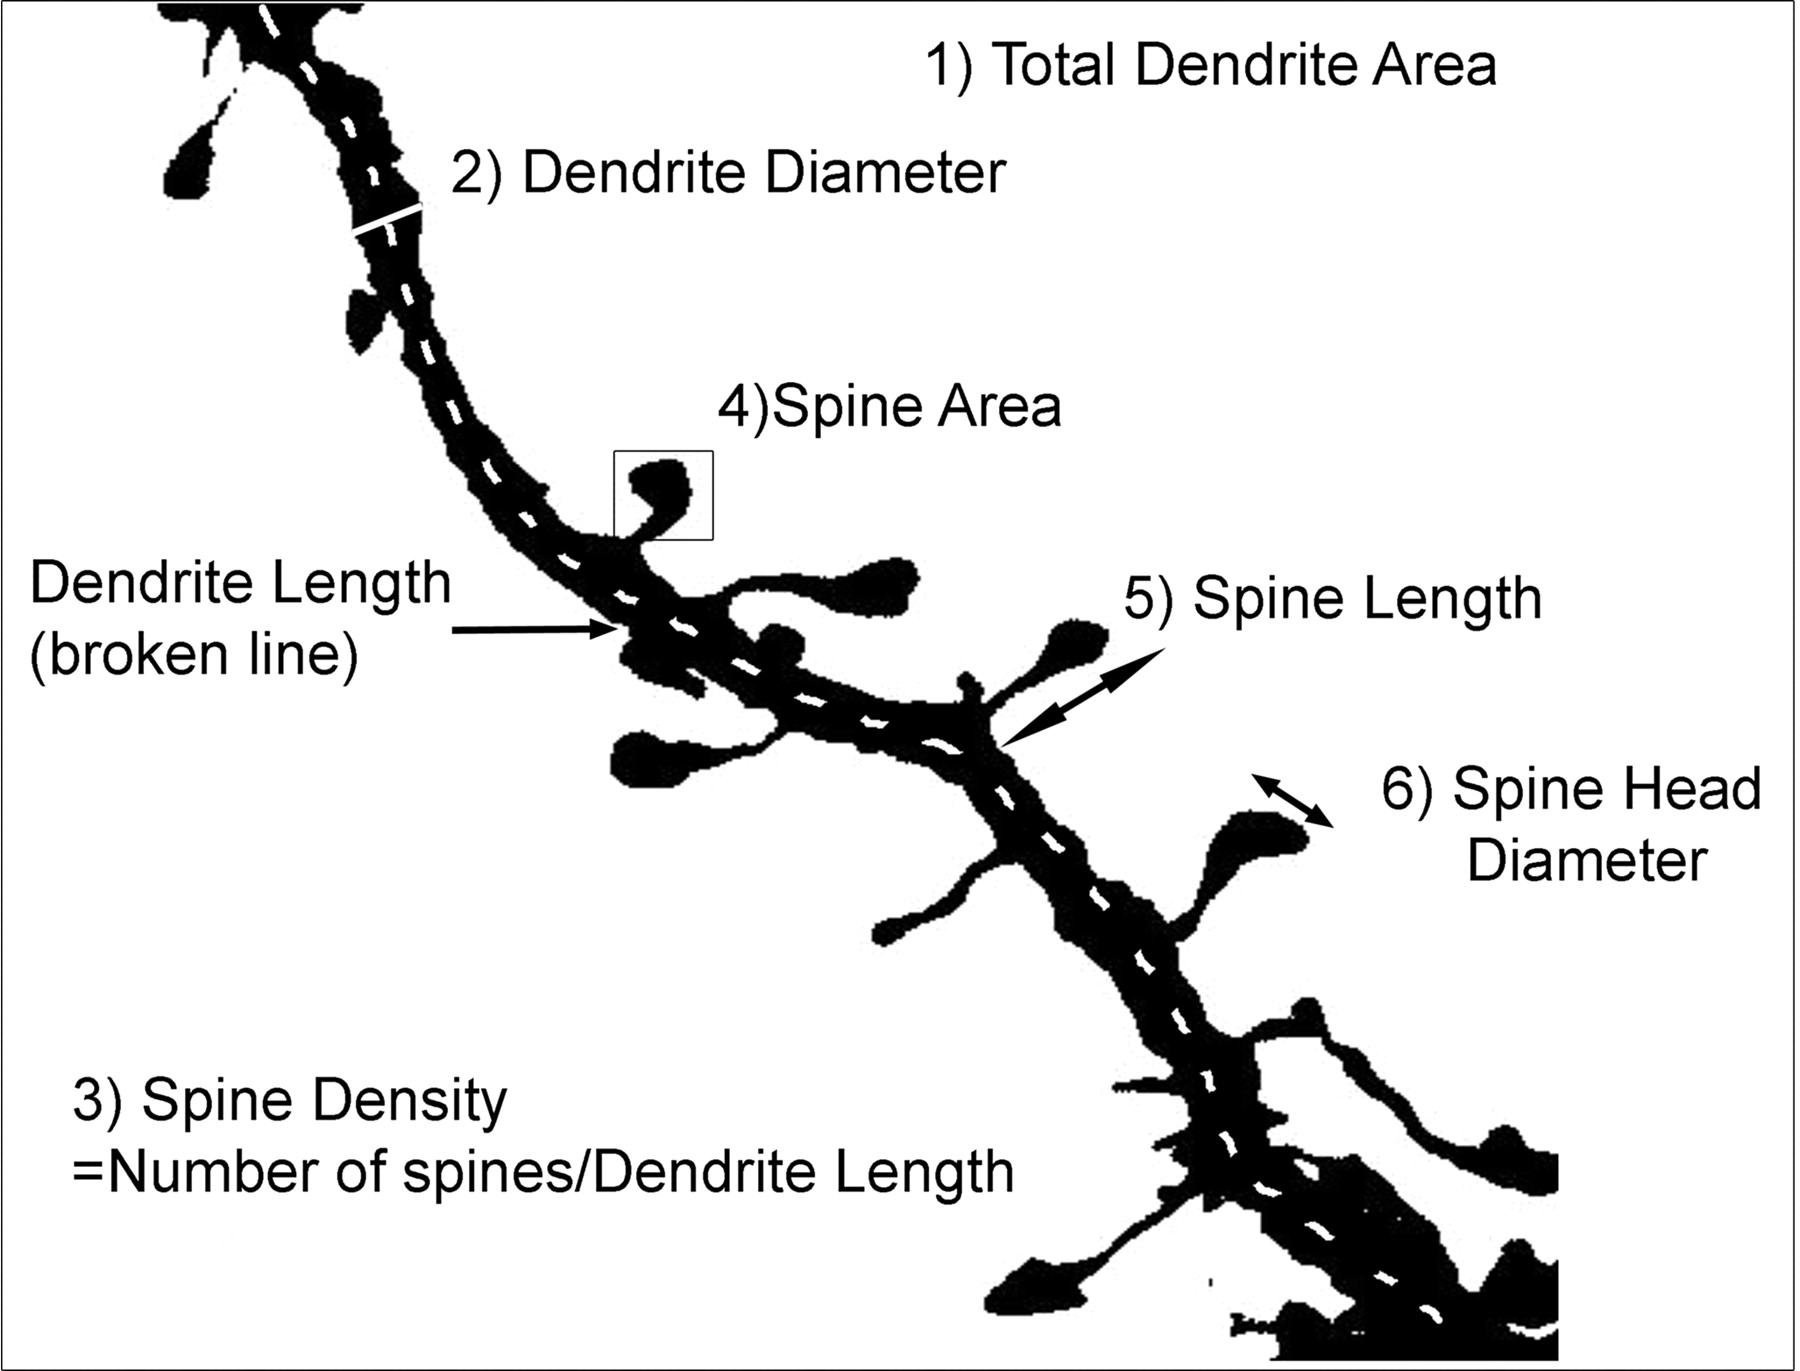
\includegraphics[scale=0.1]{../blog/images/F1_large}
    \caption{Source: Reversal of long-term dendritic spine alterations in Alzheimer disease models.
      \url{http://www.pnas.org/content/106/39/16877.abstract}.}
    \label{fig:morphometry}
\end{figure}

\end{frame}

\begin{frame}
\frametitle{Polygon meshes}

Our approach is to use polygon meshes to provide more accurate
representations of neuronal morphologies.

\pause

\begin{itemize}
\item A polygon mesh is composed of large numbers of simple polygons
  such as triangles or quads. These are stitched together to represent
  a surface.
\pause
\item In an ideal world one would want to use volumetric meshes, which
  stitch together polyhedra to fill the represented volume. However,
  at present we are only looking at surface meshes.
\pause
\item We have additional requirements on surface meshes in order for
  them to be applicable to all use cases~--- morphometry,
  reaction-diffusion, electrophysiology, etc~--- which are not needed
  for other uses such as computer graphics/games.
\end{itemize}

\end{frame}

\begin{frame}
\frametitle{Polygon meshes}

Polygon meshes are popular:

\pause

\begin{itemize}
\item The popularity of Computer Graphics and 3D Printing means that
  there are many libraries, packages and applications to choose
  from. There are also a number of file formats for meshes (OFF, STL,
  etc).
\pause
\item We want to define our own file format since we want to add
  annotations specific to neuroscience, but we also want to reuse
  existing mesh formats.
\end{itemize}

\end{frame}

\begin{frame}
\frametitle{Polygon meshes}

``Water-tight membranes from neuronal morphology files'':

\begin{itemize}
\item This is not a new idea. In particular, McDougal, Hines and
  Lytton wrote a paper\cite{mcdougal2013water} where they describe an
  approach to convert SWC files into water-tight meshes.
\pause
\item It is of course not possible to reconstruct the neuron's full
  shape from point and diameter data, the generated meshes are still
  useful because they define a plausible reconstruction without gaps
  and \emph{cul-de-sacs}.
\pause
\item Its a good starting point on the road to defining a mesh format
  because we can compare with the original SWC and there is a wealth
  of data available.
\pause
\item The end goal in the far future is to use high-resolution
  microscopy data as an input to the mesh generation process.
\pause
\item Another possibility is computer generated neurons which are
  realistic.
\end{itemize}

\end{frame}

\begin{frame}
\frametitle{Polygon meshes}

McDougal et al. define the criteria for the generated meshes:

\begin{itemize}
\item They must be physically plausible: ``the same space cannot be
  occupied by different matter, the surface must not have holes and
  the surface must not lie inside of the
  neuron.''\cite{mcdougal2013water}
\pause
\item They must be biologically plausible: ``no portion of a dendrite
  must extend past its neighbour.''\cite{mcdougal2013water}
\end{itemize}

\end{frame}

\begin{frame}
\frametitle{Polygon meshes}

Meshes must be completely manifold or watertight. This is a very
important requirement.
\pause

\begin{itemize}
\item Mathematical understanding: Non-manifolded edges are a
  problem. These are are parts of a model where the dots have not been
  connected to create a polygon. A line, or even a plane, does not have
  dimensions in three separate directions (x, y, z).
\pause
\item Intuitive understanding: if one were to fill in a physical
  representation of the model with water, would it have leaks.
\end{itemize}

\end{frame}

\begin{frame}
\frametitle{Polygon meshes}

The mesh generation process:

\begin{itemize}
\item First step: ``fix'' the SWC file, looking for
  inconsistencies such as missing parents, points with the same
  position on the plane and so on.
\pause
\item Second step: convert SWC into a CSG (Constructive Solid Geometry)
  representation. This has a number of primitives, defined by implicit
  functions. At this stage we can deal with join problems.
\pause
\item Third step: Convert the CSG representation into a mesh
  representation by polygonising/tessellating the CSG primitives. At
  this stage we can deal with affine transformations.
\end{itemize}

\end{frame}

\begin{frame}
\frametitle{Polygon meshes}

The mesh generation process (continued):

\begin{itemize}
\item Forth step: Ensure the validity of the surface by using CTNG
  (Constructed Tesselated Neuronal Geometry), which removes parts of
  the surface that lie inside of it and ensures the generation of a
  consistent, continuous surface.
\pause
\item Fifth step: Consider performing deformations to the generated
  mesh to make it more biologically plausible.
\end{itemize}

\end{frame}

\begin{frame}
\frametitle{The Processing Pipeline}

The implementation of the generation process is being done with a
processing pipeline:

\begin{itemize}
\item SWC model: simple library that reads SWC files and stores them in
  memory.
\pause
\item Geometry: simple geometry library that contains the solids
  required by SWC: spheres and frustum and ties them together with
  basic CSG operations (union) and affine transformations
  (translations, rotations).
\pause
\item Geometry.VTK: Interface to the VTK library to provide a limited
  interactive display for the generated mesh.
\end{itemize}

\end{frame}

\begin{frame}
\frametitle{The Processing Pipeline}

The responsibilities of the Geometry library are to:

\begin{itemize}
\item Convert the SWC objects into the Geometry solids (Geometry.SWC);
\pause
\item Perform a number of Affine transformations to get those solids
  in the right positions in 3D space;
\pause
\item Tesselate the solids into a polyhedra representation;
\pause
\item Convert the polyhedra representation into Nef polygons as
  supported by the CGAL library;
\pause
\item Convert the Nef representation into a CGAL mesh.
\pause
\item Produce all of the required transformations to obtain an
  water-tight mesh.
\end{itemize}

\end{frame}

\begin{frame}
\frametitle{The Processing Pipeline}

The responsibilities of the Geometry library are to:

\begin{itemize}
\item Project uses Dogen, my code generator which automatically
  generates PODs/POJOs/POCOs and related services
\pause
\item All maths-intensive code uses maths libraries: CGAL for meshes
  and possibly Eigen for linear algebra (where there are CGAL
  limitations).
\end{itemize}

\end{frame}

\begin{frame}
\frametitle{Problems}

The project as originally conceived with Ben was ``Design and
Implementation of an Extensible Representation for 3D Neuronal
Morphologies``. It has a few problems:

\begin{itemize}
\item The problem space for the entire solution is too large; creating
  a complete solution will take many man-years.
  \pause
\item There are a lot of difficult software engineering problems that
  need to be addressed but will not add value to the search towards a
  science question.
\pause
\item There are many thorny mathematical problems that need to be
  addressed in order to produce a viable mesh. My mathematical
  knowledge is insufficient to address them.
\end{itemize}

\end{frame}

\begin{frame}
\frametitle{Problems}

\begin{itemize}
\item Its a chicken and egg problem:
  \begin{itemize}
  \item no simulator is using the new file format;
    \pause
  \item the work to integrate a new file format into a
    simulator is non-trivial;
    \pause
  \item but science questions normally arise from people creating
    models and producing better (or different) results from the
    existing ones.
    \pause
  \end{itemize}
\item therefore~--- unless we do the work ourselves~--- the file
  format will not be able to bootstrap.
\pause
\item however, integrating a new file format into one of the existing
  simulators is a non-trivial task and a project in its own right
  because of the coupling between format and simulator.
\end{itemize}

\end{frame}

\begin{frame}
\frametitle{Problems}

\begin{itemize}
\item Looking back, we never had a concrete, manageable science
  question; the science question as originally defined was too vague.
  \pause
\item The idea was a bit too ambitious and its scope ill-defined.
\end{itemize}

\end{frame}

\begin{frame}
\frametitle{Towards a Solution}

I am now working on trying to address the problems above. Michael
planted the seeds of a feasible strategy:

\begin{itemize}
\item Instead of having a complete end-to-end pipeline with realistic
  meshes, we will just create any kind of vaguely suitable mesh;
\pause
\item We will then locate an existing SWC-based compartment model that
  is either stand-alone C++ code or is easy to re-implement in a
  stand-alone manner;
\end{itemize}

\end{frame}

\begin{frame}
\frametitle{Towards a Solution}

\begin{itemize}
\item We will update the model to use the mesh and attempt to
  reproduce the results; by choosing a simple model hopefully the
  integration work is also simplified.
\pause
\item Finally, we can have an end-to-end pipeline that generates some
  kind of measurable result; we can then refine it until the results
  are equal to SWC or (ideally) better.
\pause
\item The scope of the project now becomes the much less ambitious
  objective of making this pipeline working satisfactorily. However,
  the science question is dependent on the results.
\end{itemize}

\end{frame}

\begin{frame}
\frametitle{Questions?}

\end{frame}

\begin{frame}
  \printbibliography
\end{frame}

\end{document}
